\documentclass[aspectratio=169,10pt]{beamer}
\usepackage[UTF8]{ctex}\usepackage{booktabs,tabularx,graphicx,amsmath}
\definecolor{navy}{HTML}{142B43}\definecolor{teal}{HTML}{168579}
\setbeamercolor{frametitle}{bg=navy,fg=white}\setbeamercolor{structure}{fg=teal}
\setbeamercolor{block title}{bg=teal,fg=white}\setbeamercolor{block body}{bg=teal!6}
\setbeamertemplate{navigation symbols}{}\setbeamerfont{frametitle}{size=\large}
\setbeamersize{text margin left=8mm,text margin right=8mm}
\setbeamertemplate{footline}{\leavevmode\hbox{\begin{beamercolorbox}[wd=.82\paperwidth,ht=2.5ex,dp=1ex,leftskip=1em]{author in head/foot}青序量化研究平台\quad Project 2 / CogAlpha\end{beamercolorbox}\begin{beamercolorbox}[wd=.18\paperwidth,ht=2.5ex,dp=1ex,center]{date in head/foot}\insertframenumber/16\end{beamercolorbox}}}
\begin{document}

\begin{frame}{CogAlpha：让因子研发可检验}
\begin{block}{}真实模型提案，固定对照，完整保留结果\end{block}
\vspace{2mm}{\Huge\bfseries\color{navy}CogAlpha 因子研发}\par\vspace{4mm}
\small\begin{itemize}
\item Computational Finance · Project 2
\item 12412408 胡博文；12410819 谢明飞；12410436 王天希
\item 独立于RSRS路线 · 三个重复 · 约15分钟
\end{itemize}
\end{frame}
\begin{frame}{先固定问题，再看测试结果}
\begin{block}{}主比较：相同49提案槽，进化是否胜过持续提新想法？\end{block}
\small\begin{itemize}
\item 共享21个初代；两臂各新增28个槽
\item LightGBM + 测试期RankIC为固定主比较
\item 三个重复全部报告；不改选最优种子或模型
\end{itemize}
\end{frame}
\begin{frame}{从原文工作流到青序实现}
\begin{block}{}保留七层组织、质量检查、五指标与演化闭环\end{block}
\begin{center}\begin{minipage}[t]{.49\textwidth}\centering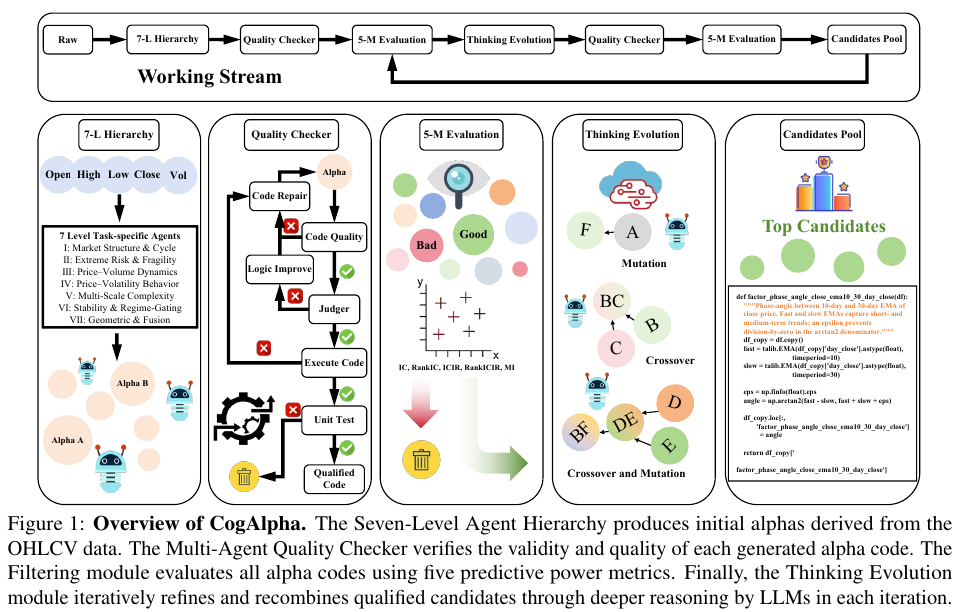
\includegraphics[width=\linewidth,height=43mm,keepaspectratio]{figures/source_figure1.png}\end{minipage}\hfill\begin{minipage}[t]{.49\textwidth}\centering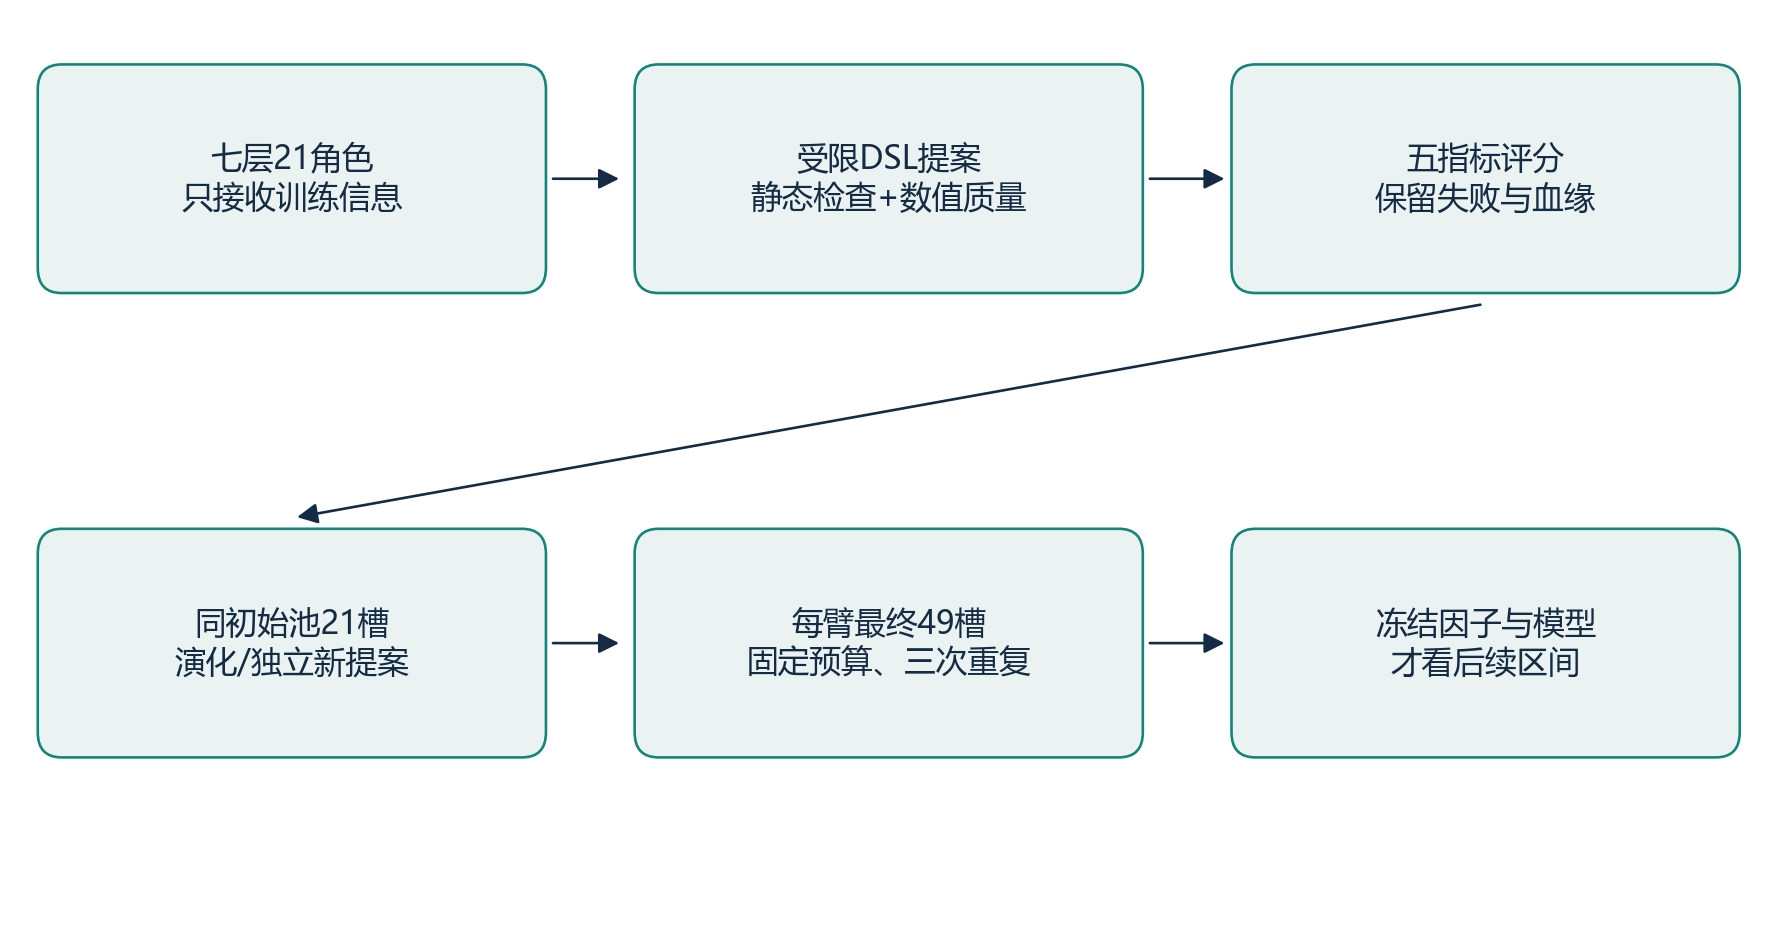
\includegraphics[width=\linewidth,height=43mm,keepaspectratio]{figures/local_workflow.png}\end{minipage}\end{center}
\small\begin{itemize}
\item 左：原文Figure 1；右：本次受限工作流
\item 不同模型、数据与搜索规模；属于机制复现
\end{itemize}
\end{frame}
\begin{frame}{时间切分与标签退出边界}
\begin{block}{}所有研发只看训练；模型先冻结，再评价后续区间\end{block}
\begin{center}
\includegraphics[width=.97\textwidth,height=42mm,keepaspectratio]{figures/split_timeline.png}\end{center}
\small\begin{itemize}
\item 训练2020—2022；验证2023—2024；测试2025—2026.09
\item 标签退出必须在下一切分前；静态股票池与已看历史仍是限制
\end{itemize}
\end{frame}
\begin{frame}{先做手算：原公式真的算对了吗？}
\begin{block}{}原文含义与公式分开检查，不能只复制经济叙述\end{block}
\[f_1=(H-C)/(V+\varepsilon),\quad f_3=\tanh\!\left(|C-O|/(VC+\varepsilon)\right)\]
\small\begin{itemize}
\item H−C是高点到收盘距离，不是C−O上涨
\item 教学输入O10/H12/L9/C11/V100000股；三式执行与手算一致
\end{itemize}
\end{frame}
\begin{frame}{生成不等于执行，更不等于交易}
\begin{block}{}模型只提公式和假设；程序决定能否进入研究池\end{block}
\small\begin{itemize}
\item OHLCV + 有限算子；单窗口\ensuremath{\le}120日
\item AST、数值覆盖率、前缀重算、未来扰动
\item 失败记录保留；一次修复仍计费
\end{itemize}
\end{frame}
\begin{frame}{同提案预算的进化消融}
\begin{block}{}每个重复77个独立槽；每个最终分支49槽\end{block}
\begin{center}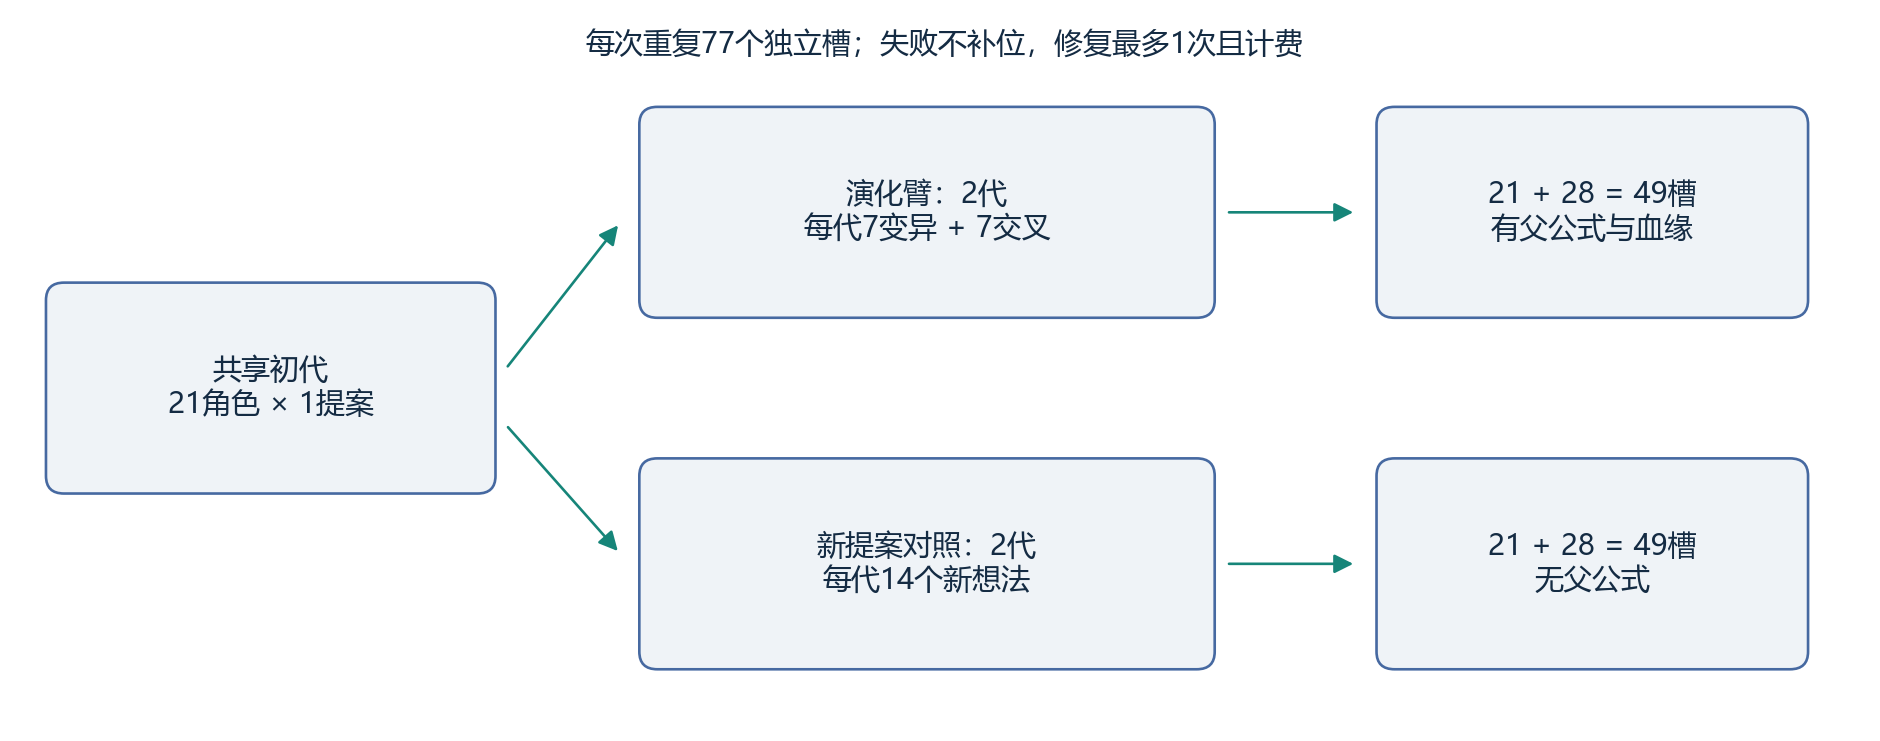
\includegraphics[width=.97\textwidth,height=42mm,keepaspectratio]{figures/matched_budget.png}\end{center}
\small\begin{itemize}
\item 实际提案请求尝试236次；失败与修复均保留
\item 新提案臂看自身训练摘要，但不接收父公式
\end{itemize}
\end{frame}
\begin{frame}{五指标资格与工程回退分开}
\begin{block}{}qualified必须五项同时达标；不能把回退池改名\end{block}
\small\begin{itemize}
\item 65\% / 80\%分位与绝对底线共同约束
\item MI为本地五分位插件估计；原估计器未公开
\item 无qualified时可用正训练RankIC回退，并明确标记
\end{itemize}
\end{frame}
\begin{frame}{主结果：三个重复完整展示}
\begin{block}{}三次重复中0/3次测试RankIC提高，平均变化-0.0068，范围-0.0109至-0.0025。\end{block}
\begin{center}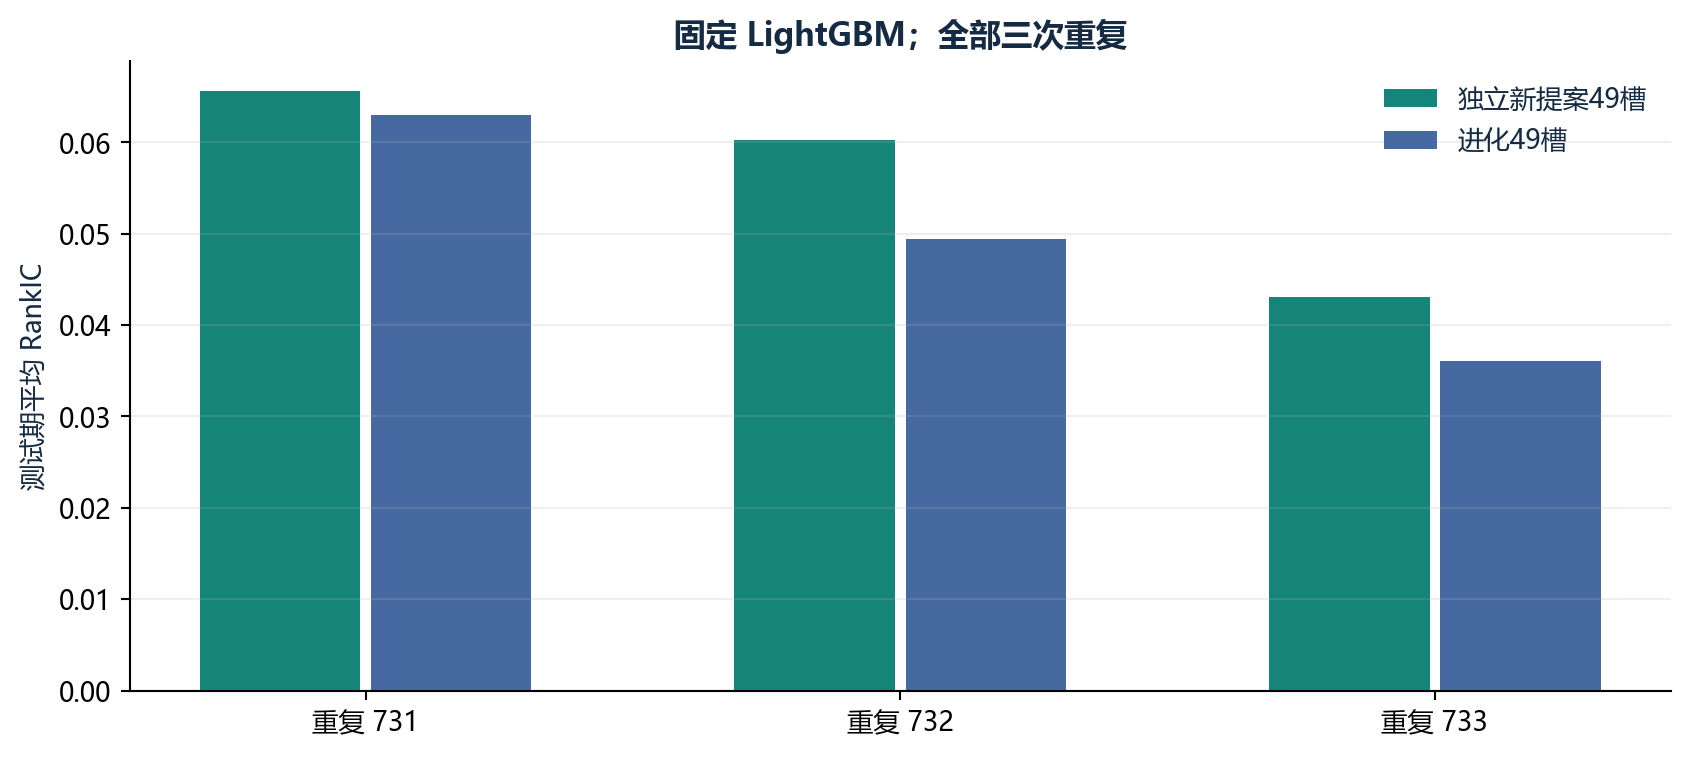
\includegraphics[width=.97\textwidth,height=42mm,keepaspectratio]{figures/primary_rankic.png}\end{center}
\small\begin{itemize}
\item 差值定义：进化减新提案；主指标为测试RankIC
\item 不据此更换主模型、种子或超参数
\end{itemize}
\end{frame}
\begin{frame}{原表与本次结果：保留条件再比较}
\begin{block}{}原文Table 1是文献基准；本次不计算直接复现误差\end{block}
\begin{center}\begin{minipage}[t]{.49\textwidth}\centering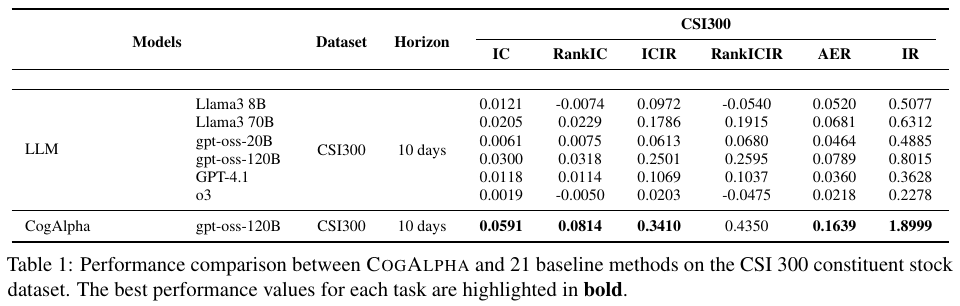
\includegraphics[width=\linewidth,height=43mm,keepaspectratio]{figures/source_table1_focus.png}\end{minipage}\hfill\begin{minipage}[t]{.49\textwidth}\centering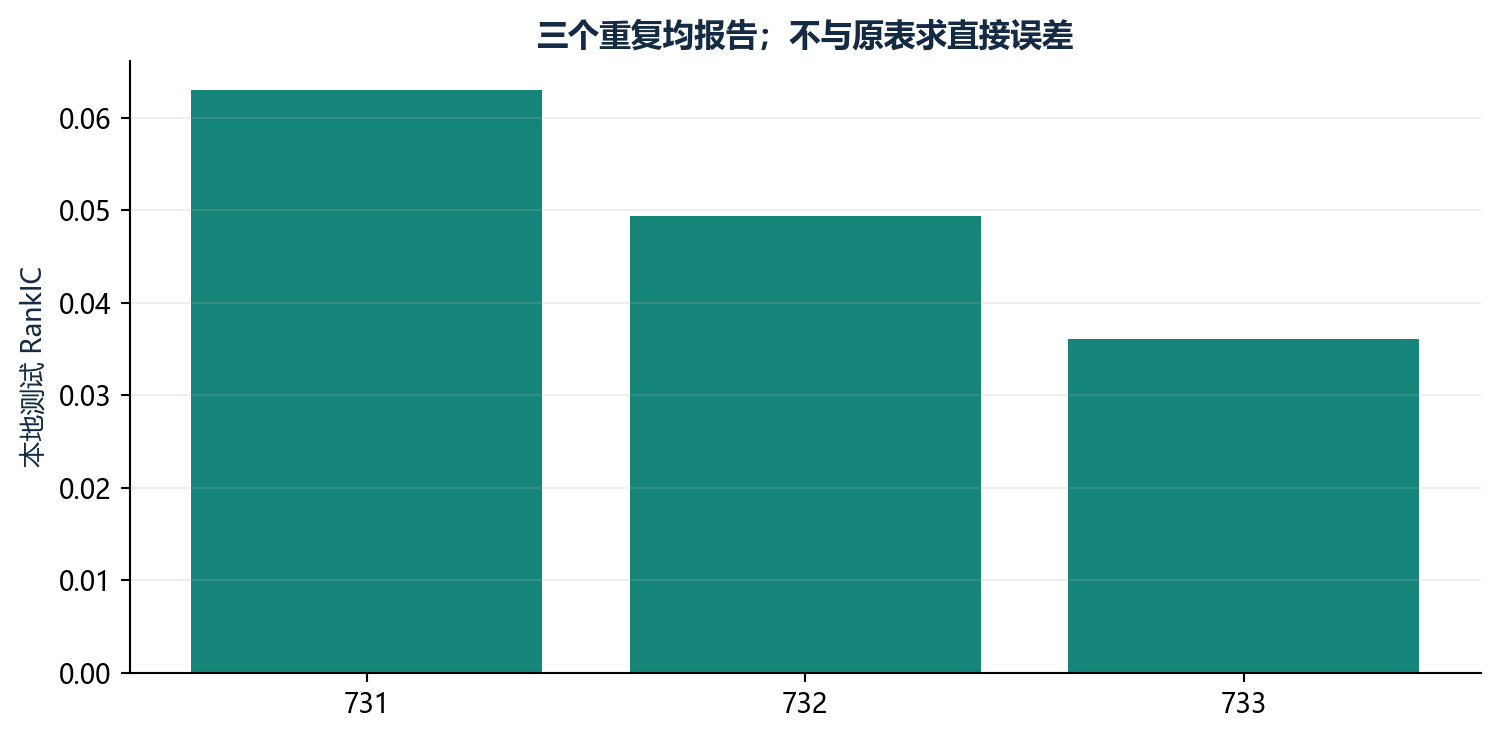
\includegraphics[width=\linewidth,height=43mm,keepaspectratio]{figures/local_table_comparison.png}\end{minipage}\end{center}
\small\begin{itemize}
\item 左：原Table 1表头与LLM/CogAlpha行摘录；中间行省略
\item 右：本次三个重复；股票池、日期、模型与训练方式均不同
\end{itemize}
\end{frame}
\begin{frame}{交易结果：排序能力之后还要核账户}
\begin{block}{}Top50/Drop5、下一开盘成交、真实费用规则\end{block}
\begin{center}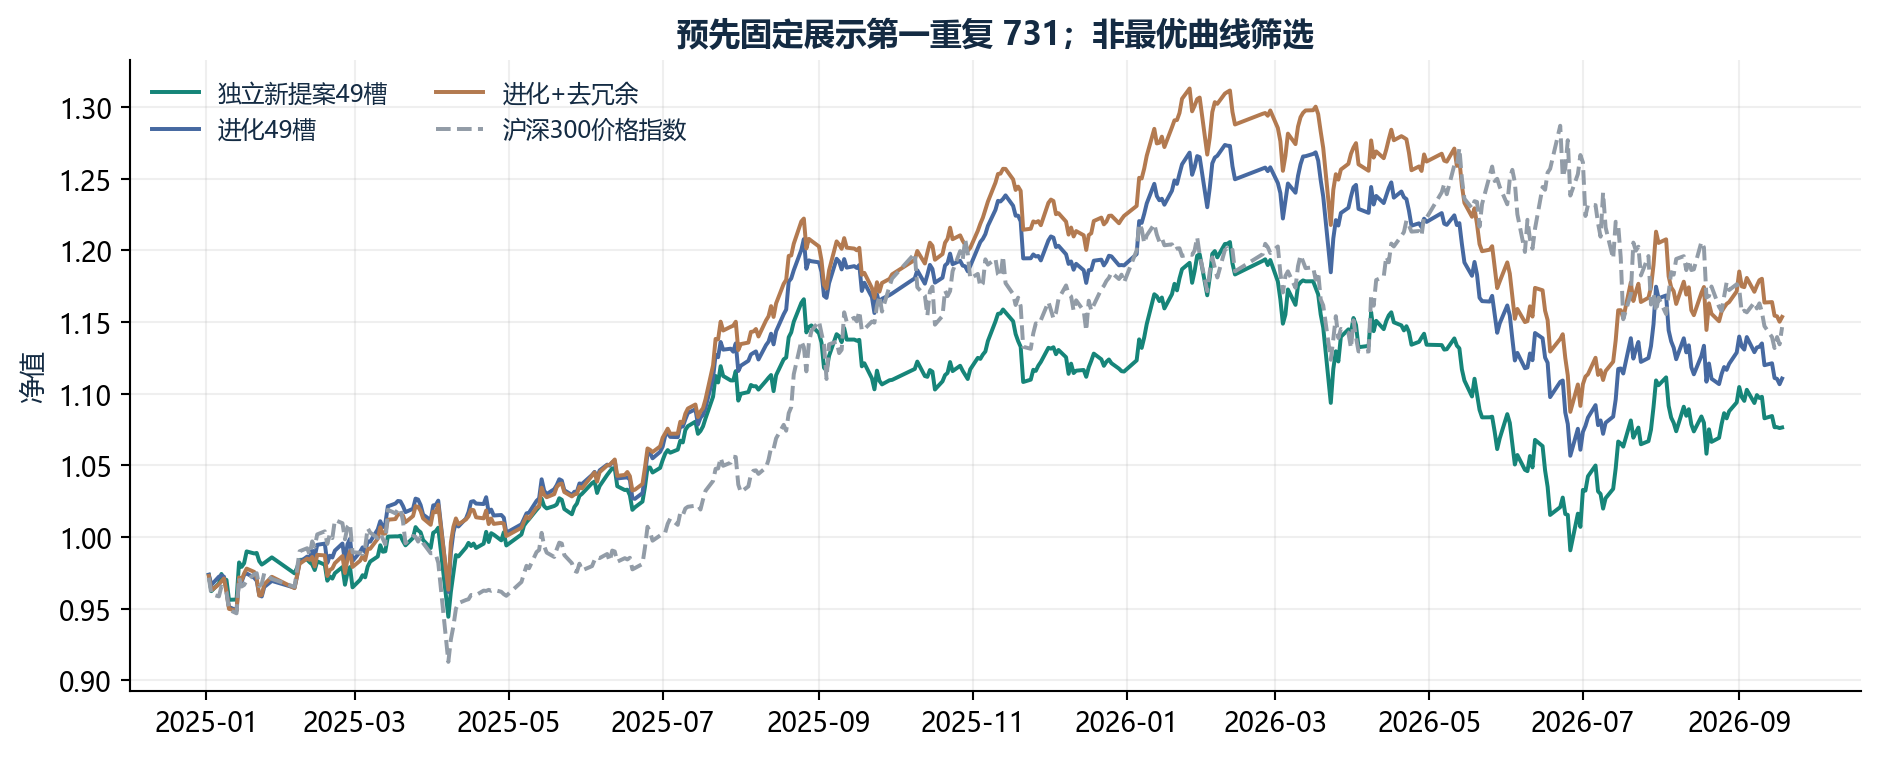
\includegraphics[width=.97\textwidth,height=42mm,keepaspectratio]{figures/portfolio_first_seed.png}\end{center}
\small\begin{itemize}
\item 预先固定展示第一重复731；报告同时列出三个重复
\item 股票复权总收益单位 vs 沪深300价格指数：分红口径不同
\end{itemize}
\end{frame}
\begin{frame}{独立改进：训练IC路径去冗余}
\begin{block}{}三次重复中2/3次测试RankIC提高，平均变化+0.0010，范围-0.0031至+0.0030。\end{block}
\begin{center}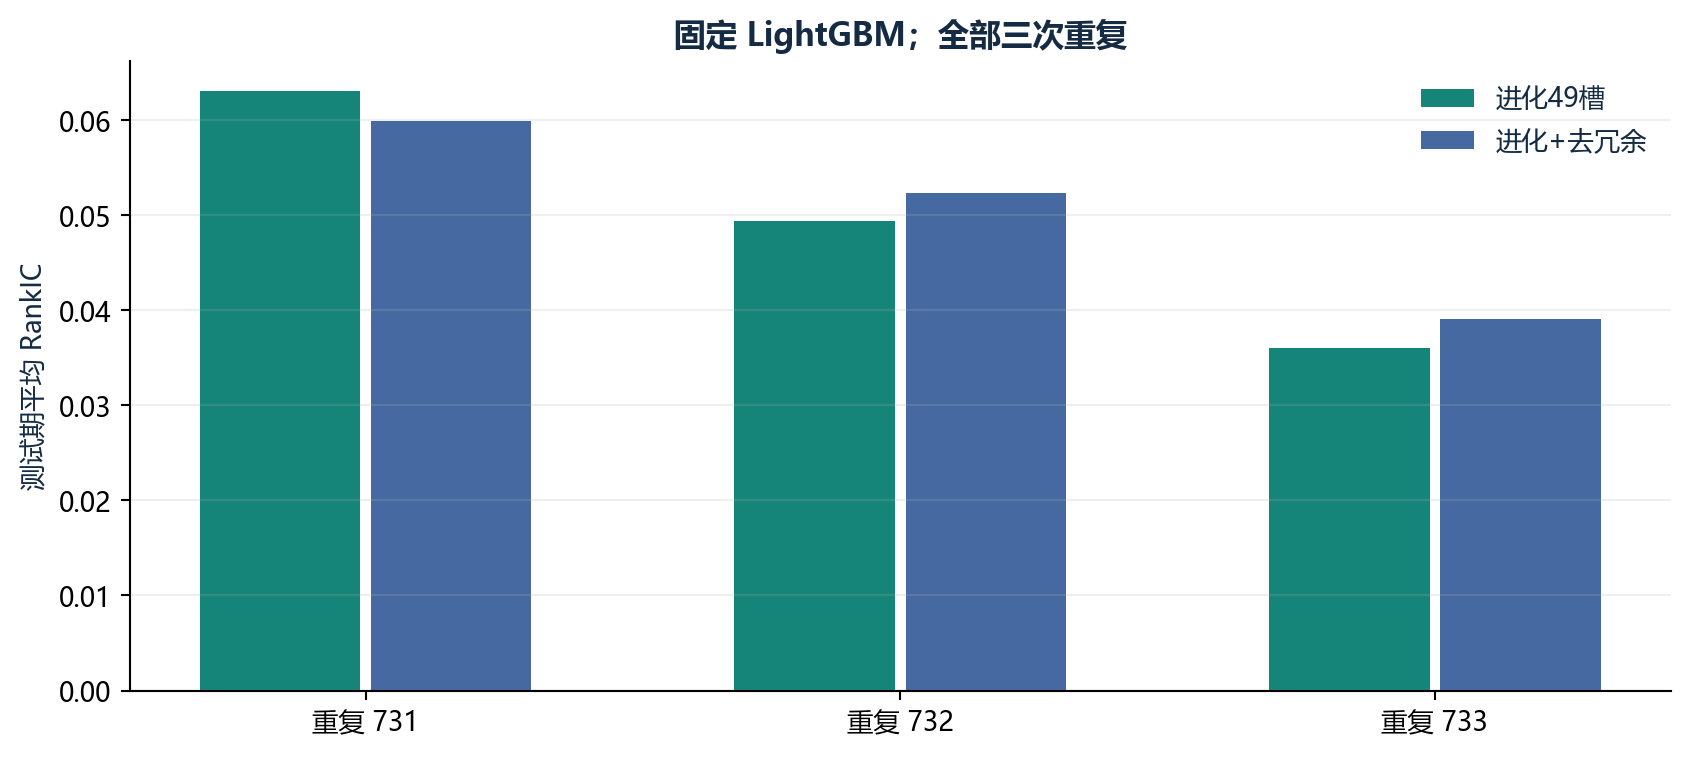
\includegraphics[width=.97\textwidth,height=42mm,keepaspectratio]{figures/diverse_rankic.png}\end{center}
\small\begin{itemize}
\item 保持进化候选池；IC路径绝对相关阈值固定0.8
\item 去冗余后最多20因子；不利用测试选阈值
\end{itemize}
\end{frame}
\begin{frame}{平台演示：从结论追到证据}
\begin{block}{}每个结果都能追溯到协议、候选公式与调用记录\end{block}
\small\begin{itemize}
\item 先选主比较：LightGBM / 测试 / 指定费用
\item 查看三个重复、失败槽、父因子与公式
\item 下载公开汇总；读取结果无需重新付费
\end{itemize}
\end{frame}
\begin{frame}{结论与限制一起保留}
\begin{block}{}我们交付可检验的研究流程；不把历史结果当作承诺\end{block}
\small\begin{itemize}
\item 静态股票池、历史已观察、LLM知识污染风险
\item 数据/模型/MI/训练方式不同，不能宣称精确原表重现
\item 下一步：冻结候选，用新的时间与成分历史验证
\end{itemize}
\end{frame}
\begin{frame}{备份：模型和收益口径}
\begin{block}{}预测指标、账户收益和成本对照各有定义\end{block}
\small\begin{itemize}
\item Ridge alpha100；LightGBM 200树/15叶/深度5/学习率0.05
\item ICIR不年化；Sharpe按252日年化，零无风险收益
\item AER为平均日超额算术年化；CAGR为复利年化
\item 最大回撤包含初始资金；整数交易与冲击仍是限制
\end{itemize}
\end{frame}
\begin{frame}{备份：来源与验收范围}
\begin{block}{}论文摘录、实验身份、原始槽位和核账记录均保留\end{block}
\small\begin{itemize}
\item 原文v4与官方提示词commit固定；裁图范围逐一记录
\item 462项去重自动测试跨已记录环境全部通过；另附独立审计器合成自检
\item 5项界面自动测试通过；最终浏览器操作验收另附记录
\item 公开聚合证据；密钥、原始行情和模型不公开
\end{itemize}
\end{frame}
\end{document}